\documentclass[border=15pt]{standalone}
\usepackage{tikz,amsmath}
\usetikzlibrary{arrows.meta}

% ========== 配色方案 ==========
\definecolor{hidFill}{RGB}{199,203,243}     % 卷积核紫色
\definecolor{hidLine}{RGB}{52,58,143}
\definecolor{inFill}{RGB}{183,224,177}       % 输入特征图绿色
\definecolor{inLine}{RGB}{32,102,32}
\definecolor{outFill}{RGB}{243,199,199}     % 输出特征图红色
\definecolor{outLine}{RGB}{143,52,52}

\begin{document}
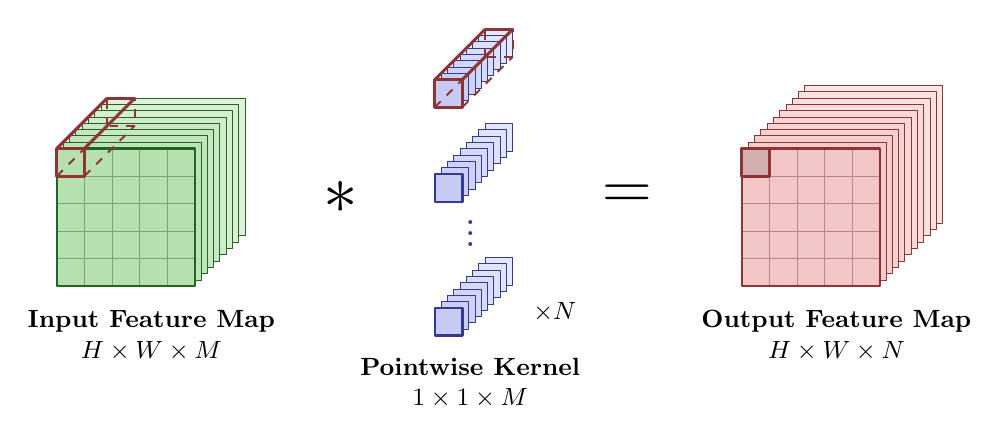
\begin{tikzpicture}[
    font=\small, line join=round,
    every node/.style={inner sep=0pt, outer sep=0pt, align=center}
  ]

  % ========== 通用 3D 堆叠切片宏 ==========
  % #1: x, #2: y, #3: 网格格数, #4: 单元格尺寸, #5: 颜色前缀, #6: 叠加层数, #7: 层间深度步长
  \newcommand{\stackbox}[7]{%
    \foreach \k in {#6,...,1}{%
      \pgfmathtruncatemacro{\op}{round(100 - (55 * \k / #6))}%
      \fill[#5Fill!\op, draw=#5Line, line width=.35pt]
            ({#1+#7*\k},{#2+#7*\k}) rectangle ++(#3*#4,#3*#4);
    }
    \fill[#5Fill] (#1,#2) rectangle ++(#3*#4,#3*#4);
    \draw[step=#4, #5Line!60, line width=.35pt, shift={(#1,#2)}] (0,0) grid (#3*#4,#3*#4);
    \draw[#5Line, thick] (#1,#2) rectangle ++(#3*#4,#3*#4);
  }

  % ========== 1x1xM 立体卷积核宏 ==========
  % #1: x, #2: y, #3: 尺寸, #4: 叠加层数, #5: 步长
  \newcommand{\pwkernel}[5]{%
    \foreach \k in {#4,...,1}{%
      \pgfmathtruncatemacro{\op}{round(100 - (55 * \k / #4))}%
      \fill[hidFill!\op] ({#1+#5*\k},{#2+#5*\k}) rectangle ++(#3,#3);
      \draw[hidLine, line width=.35pt] ({#1+#5*\k},{#2+#5*\k}) rectangle ++(#3,#3);
    }
    \fill[hidFill] (#1,#2) rectangle ++(#3,#3);
    \draw[hidLine, thick] (#1,#2) rectangle ++(#3,#3);
  }

  % ========== 红色 3D 感受野/立体包裹框宏 ==========
  % #1: x, #2: y, #3: 宽, #4: 高, #5: 深度偏移
  \newcommand{\prism}[5]{%
    \draw[outLine, dashed, line width=.7pt]
          (#1+#5,#2+#5) rectangle (#1+#5+#3,#2+#5+#4);
    \draw[outLine, line width=1.1pt]
          (#1+#5,#2+#5+#4) -- (#1+#5+#3,#2+#5+#4);
    \draw[outLine, dashed, line width=.7pt]
          (#1,#2)--(#1+#5,#2+#5) (#1+#3,#2)--(#1+#3+#5,#2+#5);
    \draw[outLine, line width=1.1pt] (#1,#2) rectangle (#1+#3,#2+#4);
    \draw[outLine, line width=1.1pt]
          (#1,#2+#4)--(#1+#5,#2+#5+#4) (#1+#3,#2+#4)--(#1+#3+#5,#2+#5+#4);
  }

  % =========================================================================
  % 1. 左侧：输入特征图 (5x5xM，绿色)
  % =========================================================================
  \stackbox{0}{-0.875}{5}{0.35}{in}{8}{0.08}
  % 红色立体虚线框覆盖贯穿所有 M 通道的 1x1xM 输入柱体
  \prism{0}{0.525}{0.35}{0.35}{0.64}
  \node[align=center] at (1.2, -1.5) {\textbf{Input Feature Map}\\$H\times W\times M$};

  % 卷积乘号 * (居中对齐于 Y = 0.25)
  \node[font=\Huge] at (3.6, 0.25) {$\ast$};

  % =========================================================================
  % 2. 中间：Pointwise 卷积核 (上2个核 -> vdots -> 下1个核)
  % =========================================================================
  % 核 3 (最下方，先绘制底层核)
  \pwkernel{4.8}{-1.5}{0.35}{8}{0.08}

  % 核 2 (中间偏上)
  \pwkernel{4.8}{0.2}{0.35}{8}{0.08}

  % 核 1 (最上方，带红色立体包裹框)
  \pwkernel{4.8}{1.4}{0.35}{8}{0.08}
  \prism{4.8}{1.4}{0.35}{0.35}{0.64}

  % 中间省略号与数量标注 x N (位于核 2 与核 3 之间，置于顶层避免任何遮挡)
  \node[font=\LARGE, hidLine] at (5.25, -0.1) {$\vdots$};
  \node[font=\small, anchor=west] at (6.05, -1.2) {$\times N$};

  % 卷积核底部标签 (与两侧标签基线严格对齐)
  \node[align=center] at (5.25, -2.1) {\textbf{Pointwise Kernel}\\$1\times 1\times M$};

  % 等号 = (居中对齐于 Y = 0.25)
  \node[font=\Huge] at (7.25, 0.25) {$=$};

  % =========================================================================
  % 3. 右侧：最终输出特征图 (5x5xN，红色)
  % =========================================================================
  \stackbox{8.7}{-0.875}{5}{0.35}{out}{10}{0.08}
  % 左上角高亮单个映射输出像素点 (与左侧输入及核 1 的位置严格水平对齐)
  \fill[outLine!40] (8.7, 0.525) rectangle ++(0.35, 0.35);
  \draw[outLine, line width=1.1pt] (8.7, 0.525) rectangle ++(0.35, 0.35);
  \node[align=center] at (9.9, -1.5) {\textbf{Output Feature Map}\\$H\times W\times N$};

\end{tikzpicture}
\end{document}